%configure document, you can use a template according to the journal, enterprise, etc...
%\documentclass[11pt, letterpaper, twocolumn]{article}
\documentclass[12pt]{report} 

%%you can call packages here 
\usepackage[utf8]{inputenc} %utf8 text character encoding
\usepackage{cite}
\usepackage{amsmath,amssymb,amsfonts,nccmath}
\usepackage{hyperref}
\hypersetup{colorlinks,linkcolor={blue},citecolor={blue},urlcolor={red}}  
\usepackage{cleveref} %Para usar crefrange
\usepackage{algorithm,algorithmic}
\usepackage{graphicx}
\usepackage{textcomp}
\usepackage[font=footnotesize,labelfont=bf]{caption}
\usepackage[font=footnotesize,labelfont=bf]{subcaption}
\usepackage{graphicx}
\usepackage{color}
\usepackage{gensymb}
\usepackage{dblfloatfix}
\usepackage{lineno}
\usepackage{enumitem}
\usepackage[autostyle]{csquotes}
\usepackage{titlesec}
\usepackage[T1]{fontenc}
\usepackage{listings}
\usepackage{color}

\newcommand{\squeezeup}{\vspace{-3mm}}
% the following package is optional:
\usepackage{latexsym}

\titleformat{\chapter}[hang]
{\bfseries\huge}{Capítulo \thechapter.}{0.5em}{}


\title{Práctica 1: Implementación de un Sniffer}
\author{Rojas Ian \thanks{Student at UPIITA-IPN, Email: ian.rojas.gomez.01@gmail.com }}

\begin{document}
	\setlength{\parindent}{0pt}
	\begin{titlepage}
		
		\begin{figure}[t]
			\raggedright
			\begin{minipage}{0.5\textwidth}
				\raggedright
				{
\includegraphics[width=0.5\textwidth]{images/upiita-logo.png}\par}
			\end{minipage}%
			\raggedleft
			\begin{minipage}{0.5\textwidth}
				\raggedleft
				{
\includegraphics[width=0.5\textwidth]{images/logo-ipn.png}\par}
			\end{minipage}%
		\end{figure}
		
		\vspace{1cm}
		\centering
		{\LARGE Instituto Polit\'ecnico Nacional \par}
		\vspace{1cm}
		{\scshape\Large Unidad Profesional Interdisciplinaria de Ingenier\'ia y Tecnolog\'ias Avanzadas \par}
		\vspace{3cm}
		{\scshape\Huge \textbf{Práctica 1: Implementación de un Sniffer.} \par}
		\vfill
		{\Large \textbf{Alumno:} \par}
		{\Large Rojas Gómez Ian\par}
		\vspace{0.45cm}
		{\Large \textbf{Grupo:} 2TM8\par}
		{\Large \textbf{Profesor:} Enriquez Ortiz Cyntia Eugenia\par}
		{\Large \textbf{Unidad de Aprendizaje:} Protocolos de Internet. \par}
		{\Large \textbf{Fecha de Entrega:} Martes 22 de Febrero del 2022.\par}
		
	\end{titlepage}

	\section*{Introducción}
	
	La evolución de Internet ha traído grandes avances a la tecnología así como una comunicación rápida y eficiente, pero para que todo esto sea posible, se tuvieron que crear estándares y reglas para que la comunicación entre las computadoras fuera lo mas claro y rápido posible, a pesar de que solo requerimos un cable para poder estar conectados a lared, va mas allá de eso, que detrás de tanta simpleza se tenga un mundo fascinante. Si bien los datos que transmitimos se tienen que enviar en tramas o paquetes de datos, a continuación se van a explicar los paquetes mas utilizados en el mundo de la informática.
	
	\subsection*{Ethernet}
	En una red Ethernet los dispositivos se intercambian paquetes de datos entre sí, los llamados paquetes Ethernet. En su contenido se incluye la trama Ethernet (a menudo denominada también trama de datos), que a su vez se divide en varios conjuntos de datos. Estos registros consisten en código binario que proporciona información importante, incluyendo direcciones, información de control, datos de uso y sumas de comprobación. Dependiendo del estandar, este puede variar en su estructura, y puede contener mas o menos campos de datos dependiendo del protocolo de Red.
	
	\subsection*{Ethernet II}
	
	Una trama Ethernet debe tener al menos 64 bytes para que funcione la detección de colisiones y pueda tener un máximo de 1518 byte. Se define de la siguiente manera:
	
	\begin{enumerate}
		\item Se comienza con un preámbulo, que controla la sincronización entre el emisor y el receptor y un Start Frame Delimiter (SFD), que define la trama.
		\item Se contienen las direcciones de origen y destino en formato MAC.
		\item SE contiene la información de control (En el caso de Ethernet OO el campo de tipo, una especificación de longitud)-
		\item Seguida por un registro de datos que se envía.
		\item Una secuencia de comprobación de trama (FCS) que es un código de errores que cierra la trama.
	\end{enumerate}

	Ethernet II utiliza la estructura de trama clásica con un campo de tipo (Type) que define varios protocolos en la capa de red. La trama Ethernet II se definió en 1982 y ha constituido la base de todos los desarrollos posteriores de tramas. Sin embargo, el formato sigue gozando de gran popularidad, sobre todo porque ofrece al campo de datos una gran cantidad de espacio (hasta 1 500 bytes).
	
	\begin{figure}[!h]
		\centering
		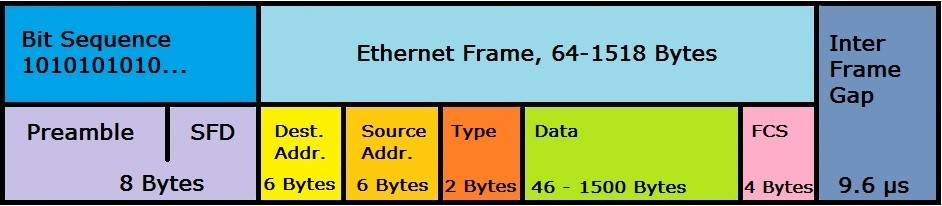
\includegraphics[width=10cm]{images/etii_structure.jpg}
		\caption{Trama Ethernet II.}
	\end{figure}

	\subsection*{IEEE 802.3}
	Esta versión estandarizada de la trama Ethernet 802.3 puede definir hasta 256 protodolos compatibles . Además, se incluyen "Punto de acceso al servicio de destino" (DSAP) y "Punto de acceso al servicio de origen" (SSAP) y el nuevo campo de control define el "Logical Link" (LLC) del protocolo.
	
	Ethernet IEEE 802.3 es la estrucutra de trama LAN  más popular y ampliamente utilizada en la actualidad.
	\cite{web:ethernet}
	
	\begin{figure}[!h]
		\centering
		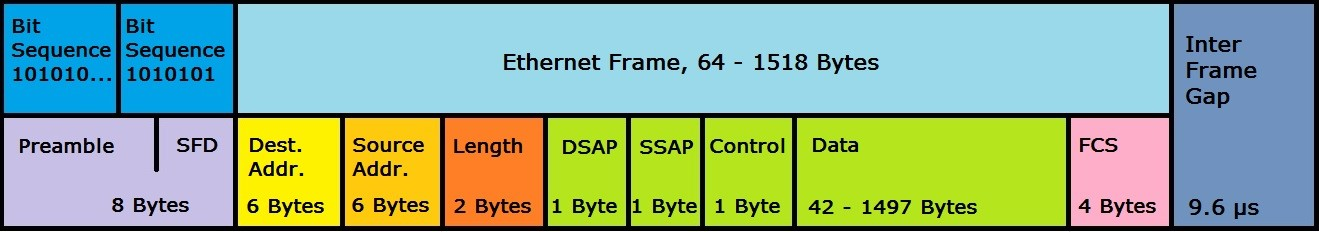
\includegraphics[width=10cm]{images/eth8023.jpg}
		\caption{Trama de Ethernet IEEE 802.3.}
	\end{figure}

	\subsection{Tecnologías de transmisión}
	Las tecnologías de tranmisión son parte fundamental debido a que las tramas deben tenerlas para saber que tipo de protocolo seguir y procesar. Existen 3 tipos de tecnologías básicas para las tramas Ethernet:
	
	\begin{itemize}
		\item \textbf{Broadcast(Difusión)}: Es la transferencia de información desde un nodo emisor a una multitud de nodos receptores. \cite{web:broadcast}
		\item \textbf{Unicast (Unidifusión)}: Es la tranferencia que se realiza desde un único emisor a un único receptor, sin importar si tiene lugar en ambas direcciones. \cite{web:unicast}
		\item \textbf{Multicast (Multidifusión)}: Se refiere a la entrega de la información a multiples destinos. \cite{web:multicast}
	\end{itemize}

	\subsection*{Modo promiscuo}
	Después de fundamentarnos acerca de lo que vamos a estar analizando en nuestro sniffer, hay que tener en cuenta una configuración de nuestra NIC que sería el \textbf{Modo Promiscuo}.
	
	El \textbf{Modo Promiscuo} es una configuración de NIC que pasa todos los paquetes al conttrolador del adaptador de red y a la plia de protocolos. Es compatible con muchos adaptadores de red cablados e inalámbricos y sus controladores. Esto va a permitir que nuestra máquina este a la escucha de todos los paquetes que esten pasando por la red, aunque dichos paquetes no sean para nosotros. \cite{web:promiscuo}
	
	\subsection*{Sniffer}
	
	Un Sniffer es una aplicación especial para redes informáticas (un software) que se encarga de capturar y analizar paquetes en tránsito (entrada y/o salida) en una red de comunicaciones entre dispositivos.
	
	Sniffer, del inglés sniff: olfatear, rastrear, puede entenderse como un programa con la capacidad de observar el flujo de datos en tránsito por una red, y obtener información de éste; está diseñado para analizar los paquetes de datos que pasan por la red y no están destinados para él, lo que bajo ciertas circunstancias es muy útil, y bajo otras, a la vez, muy peligroso.\cite{web:sniffer}
	
	\section*{Documentación}
	A continuación se van a mostrar unos diagramas realizados en UML donde se puede apreciar como se desarrollo el programa. Si bien no estan enfocados al 100\% al modelado UML sirvieron para el entendimiento del desarrollo.
	
	\begin{figure}[!h]
		\centering
		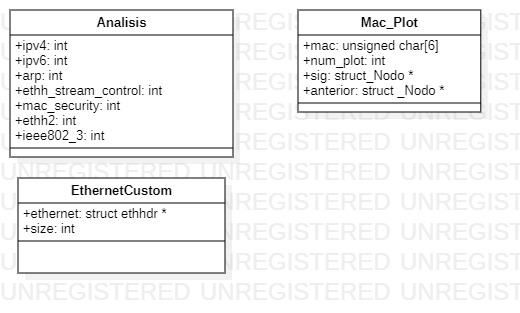
\includegraphics[width=10cm]{images/structs.jpg}
		\caption{Estructuras utilizadas para almacenar datos y facilitar el desarrollo.}
	\end{figure}
	
	\begin{figure}[!h]
		\centering
		\begin{tabular}{cc}
			
			\begin{subfigure}{0.4\textwidth}
				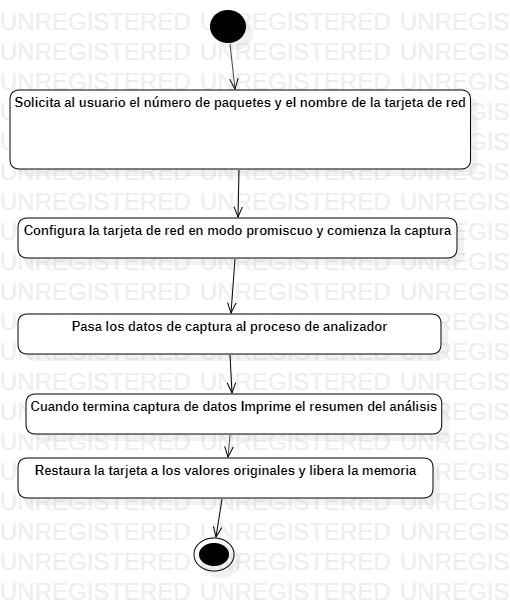
\includegraphics[width=5cm]{images/capturador.jpg}
				\subcaption{Diagrama del proceso capturador.}
			\end{subfigure}
			&
			\begin{subfigure}{0.4\textwidth}
				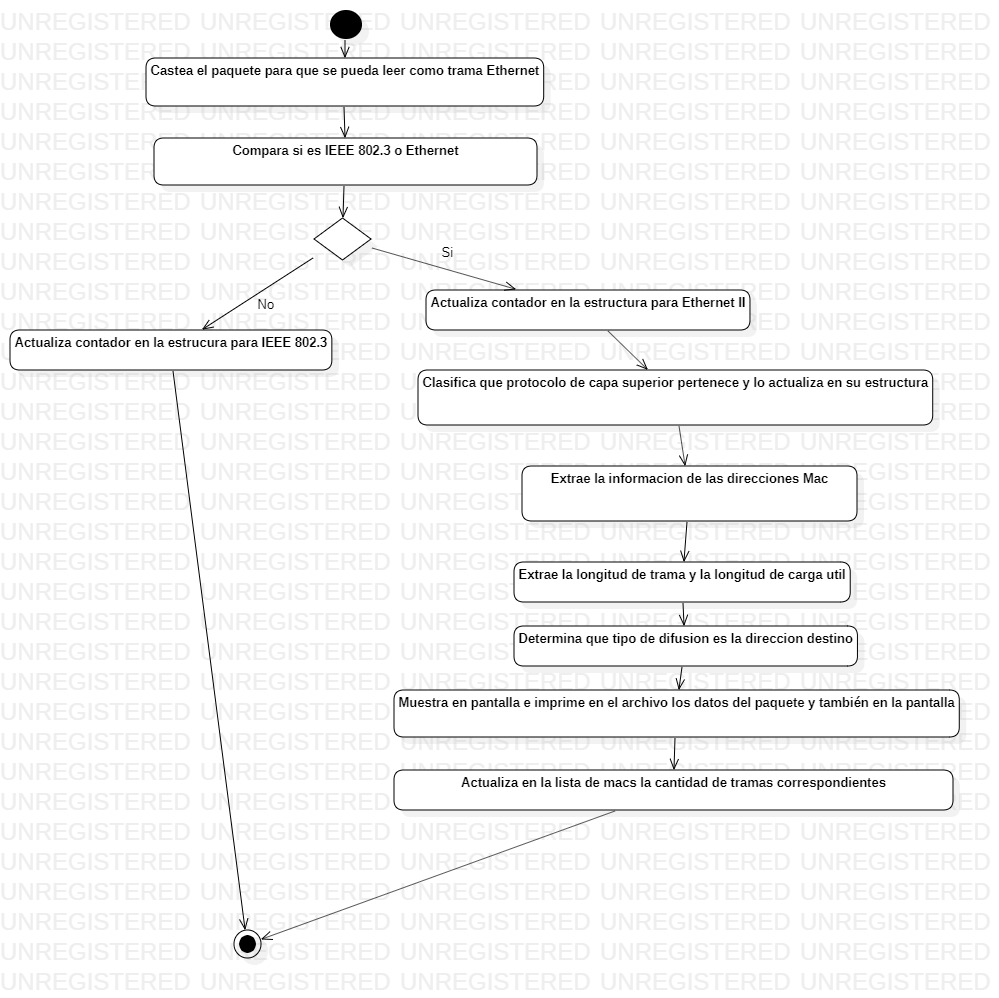
\includegraphics[width=5cm]{images/analyzer_secuence.jpg}
				\subcaption{Diagrama del proceso analizador.}
			\end{subfigure}
			
		\end{tabular}
		\caption{Diagramas de estado de los dos procesos que van a estar definiendo la funcionalidad del sniffer.}
	\end{figure}
	
	\begin{figure}[!h]
		\centering
		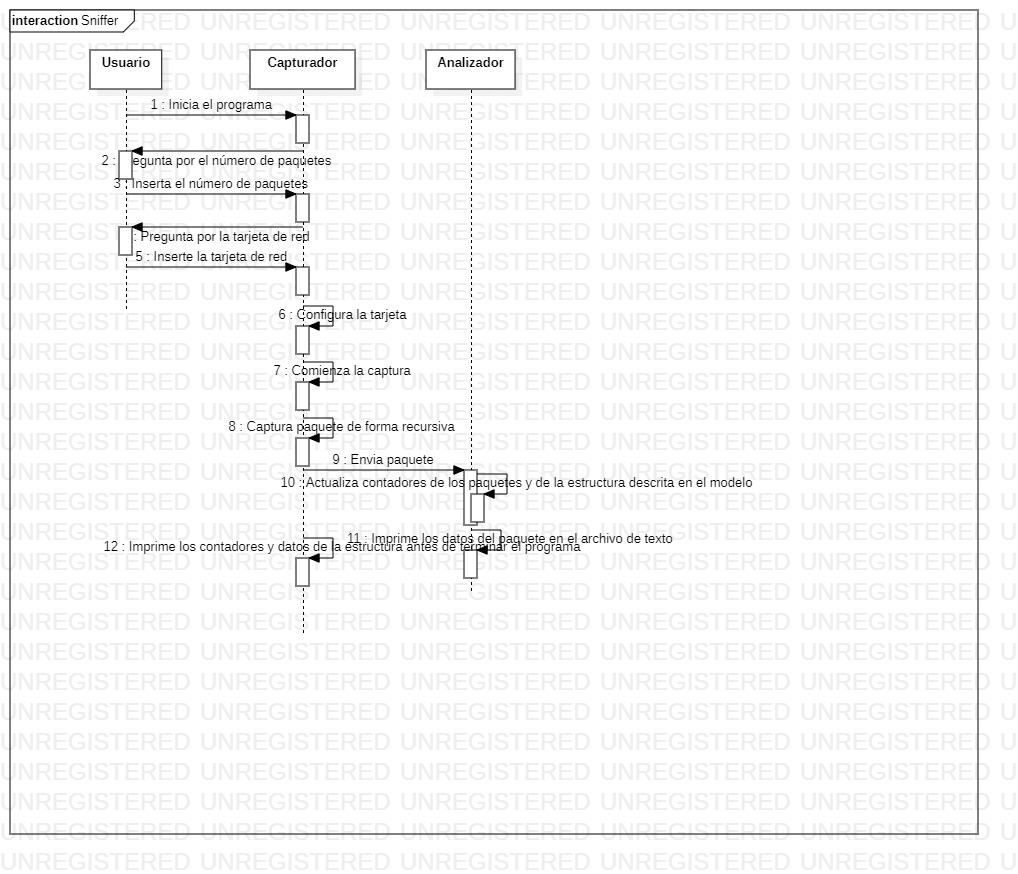
\includegraphics[width=10cm]{images/secuence.jpg}
		\caption{Diagrama de secuencia de convivencia entre el usuario, el proceso capturador y el proceso analizador.}
	\end{figure}
	
	\section*{Resultados}
	
	A continuación se van a mostrar los datos obtenidos de un análisis de 20 paquetes.
	
	\begin{figure}[!h]
		\centering
		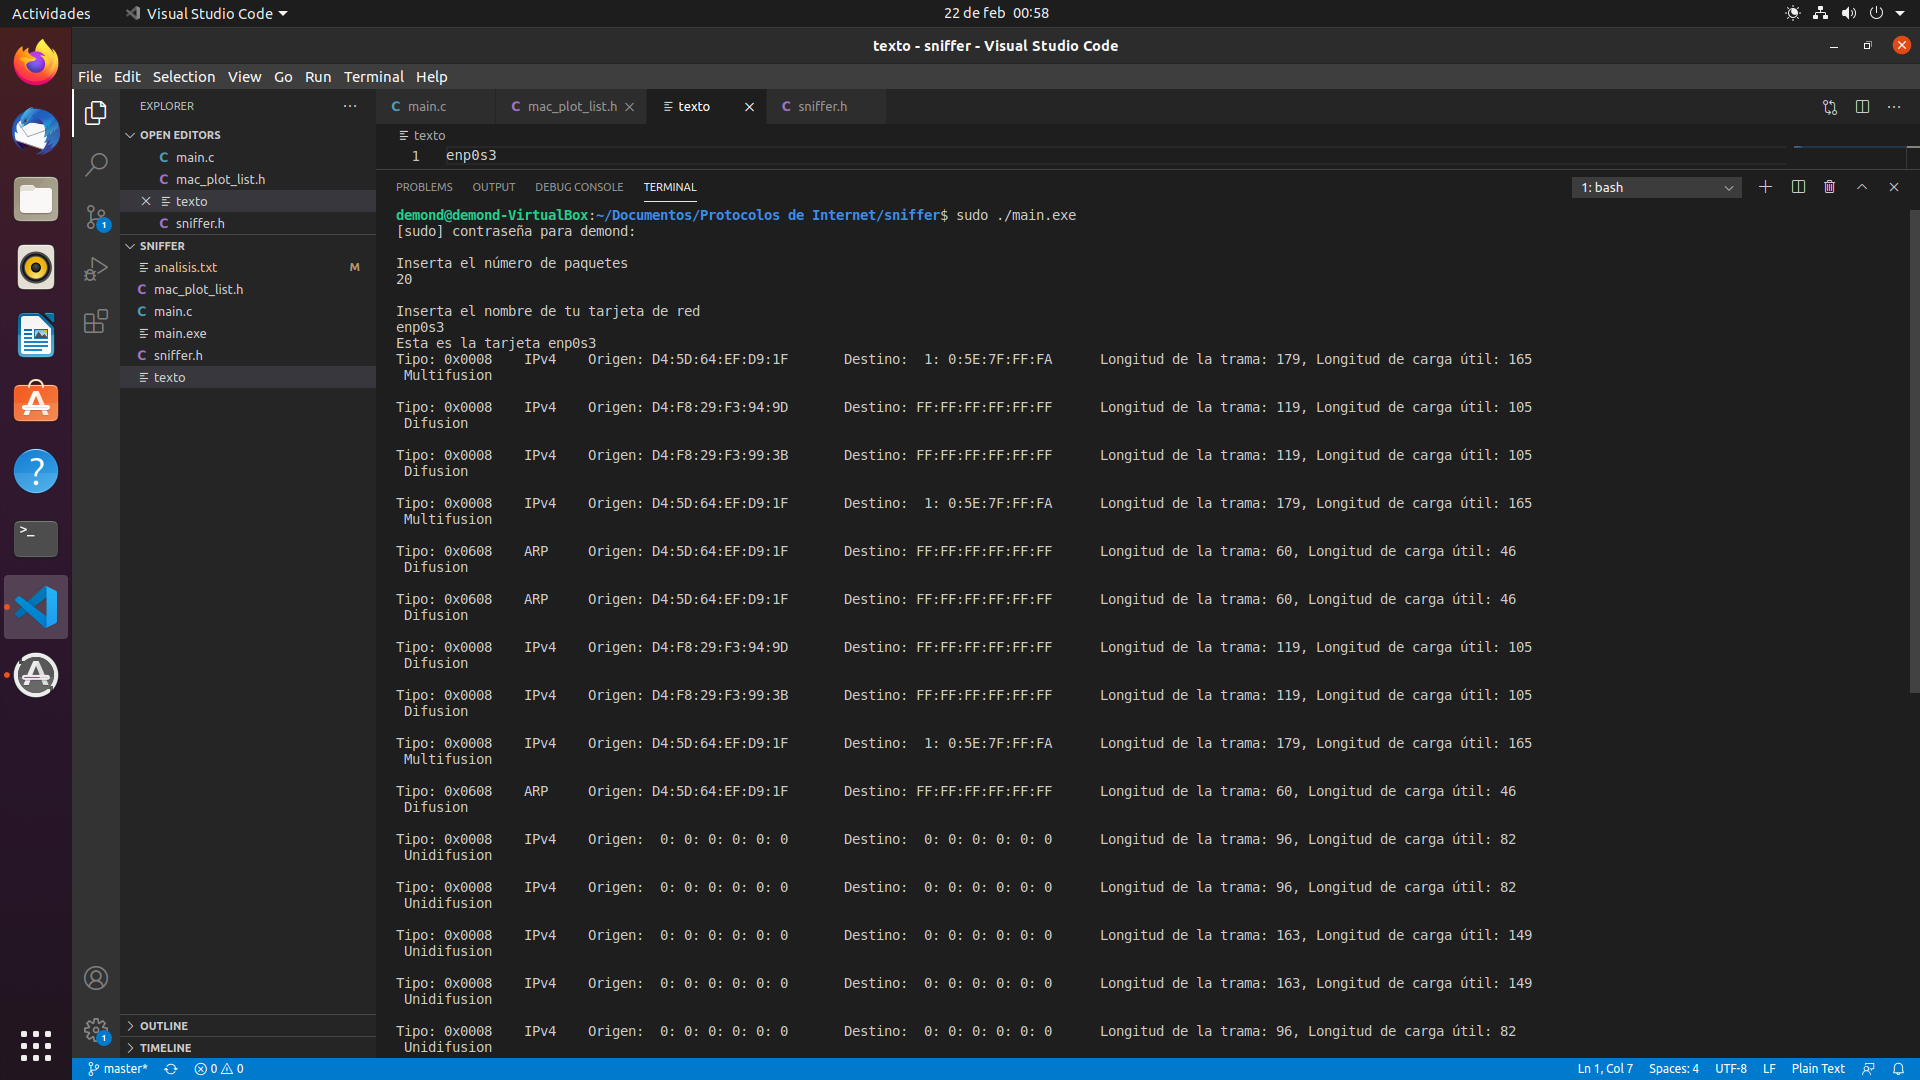
\includegraphics[width=10cm]{images/prueba1.png}
		\caption{Análisis de 20 paquetes.}
	\end{figure}

	\begin{figure}[!h]
		\centering
		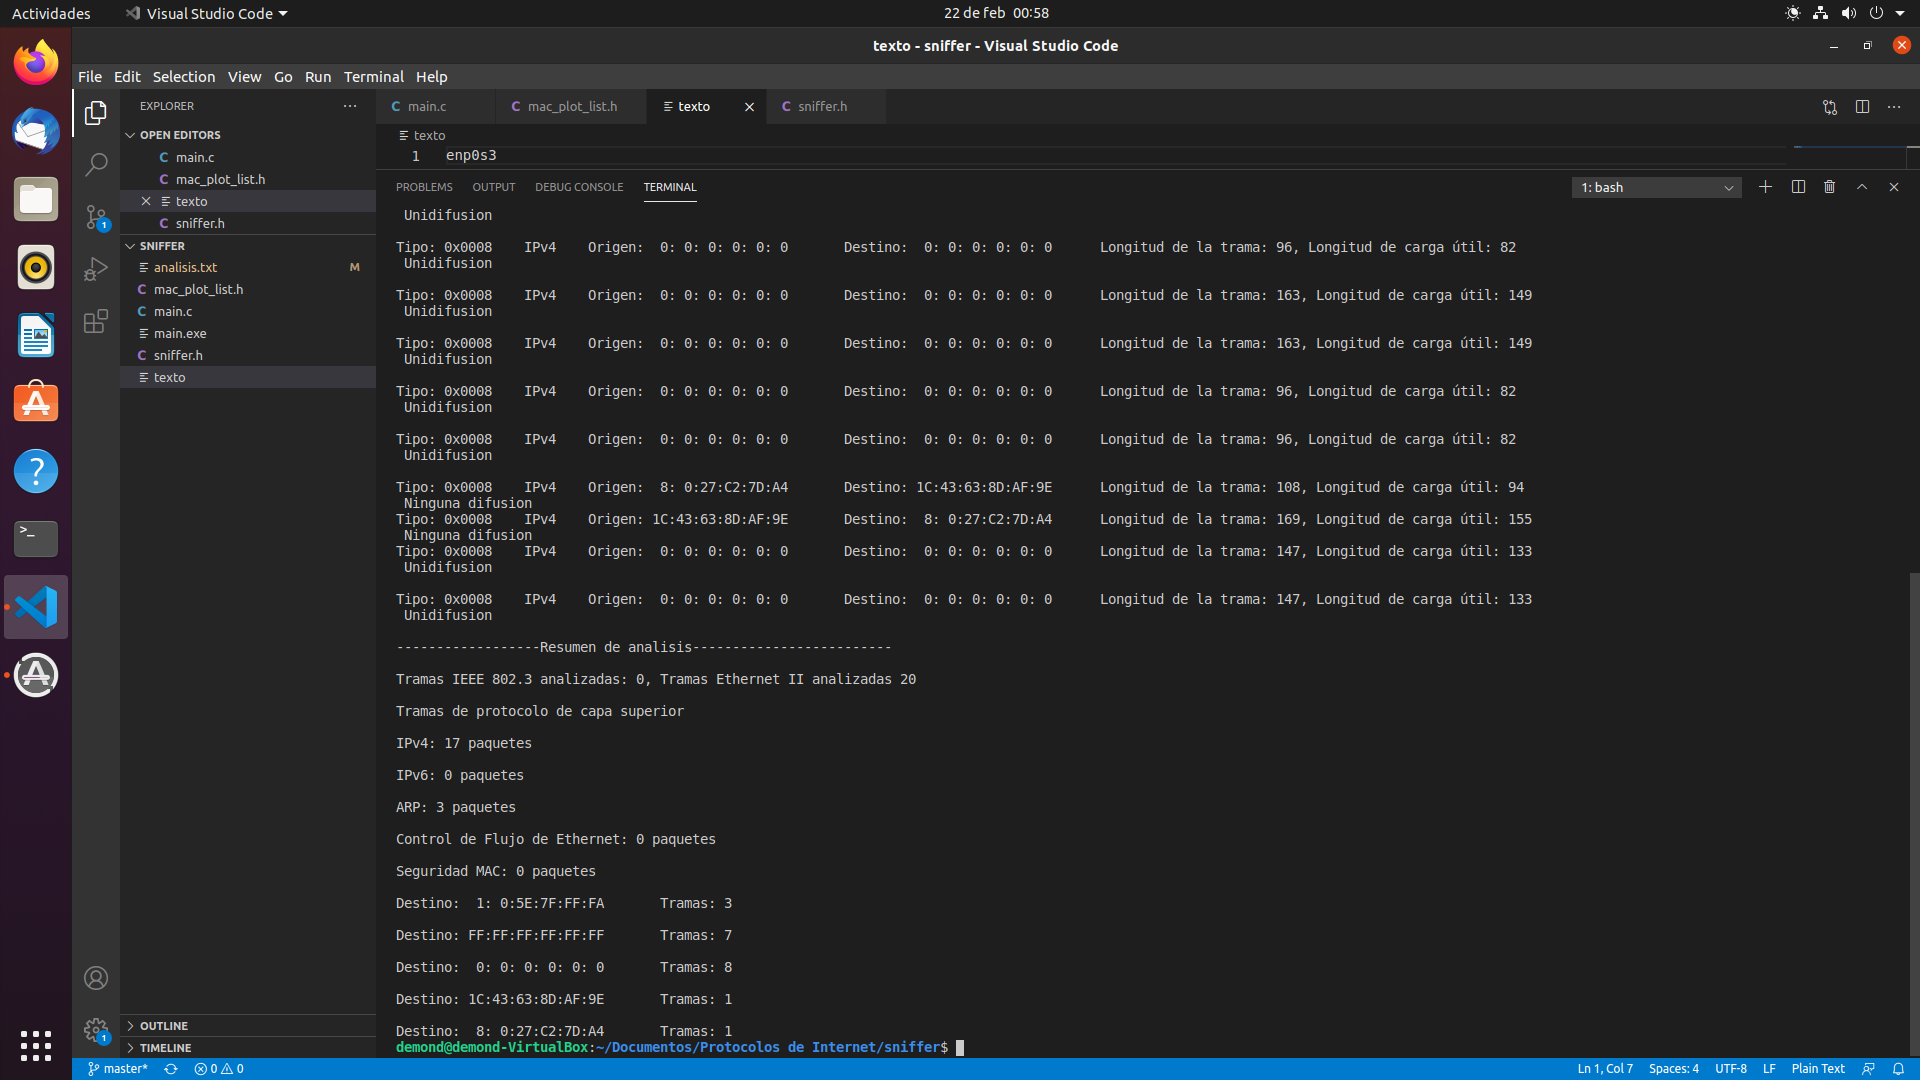
\includegraphics[width=10cm]{images/prueba1.1.png}
		\caption{Resumen de análisis de 20 paquetes.}
	\end{figure}

	\begin{figure}[!h]
		\centering
		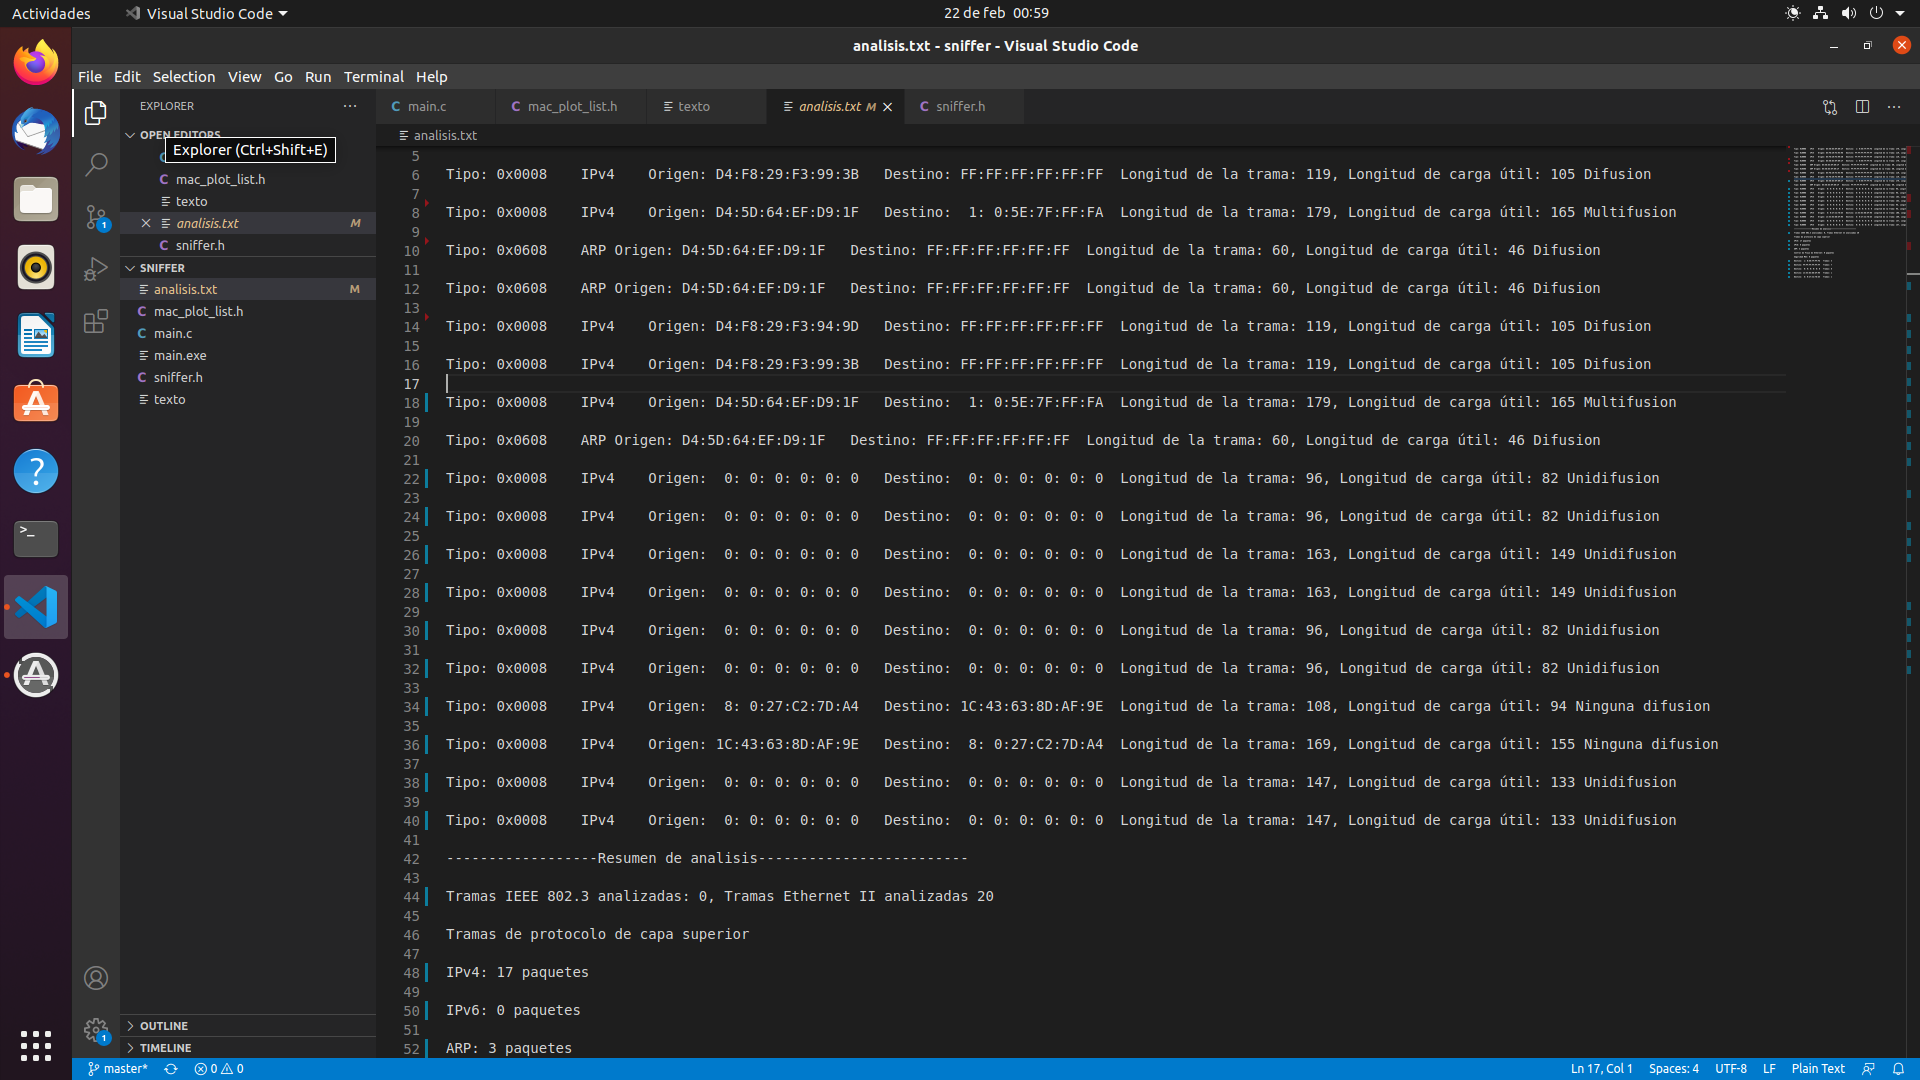
\includegraphics[width=10cm]{images/prueba2.png}
		\caption{Generación de archivo.}
	\end{figure}
	
	
	
	\bibliographystyle{ieeetran}
	\bibliography{Referencias}

\end{document}